\section{Programmation}
\begin{frame}
    \frametitle{Compilation}
\begin{block}{Un dialecte de C/C++}
    \begin{itemize}
        \item<+-> Le GPU se programme en C/C++ avec des directives spécifiques reconnues par nvcc, le 
        compilateur de NVIDIA.
        \item<+-> Placées devant un nom de variable ou de fonction, elles permettent d'en spécifier l'emplacement.
        \item<+-> Le fichier devant être compilé avec nvcc doit avoir l'extension \texttt{.cu}.
        \item<+-> CMake reconnaît CUDA comme un langage à part entière, détecte l'environnement de développement NVIDIA, et génère les projets en conséquence.
    \end{itemize}
\end{block}
\end{frame}
\begin{frame}
    \frametitle{Directives d'exécution}
    \renewcommand{\arraystretch}{2}
    \vskip 20pt
    \begin{tabular}{|c|c|}
        \hline
        \rowcolor{lightgray} Directive & Effet \\ \hline
        \_\_global\_\_ & \begin{minipage}{0.8\textwidth}
            La fonction est un noyau. Elle est compilée pour le GPU, mais peut être appelée depuis le CPU. 
        \end{minipage} \\ \hline
        \_\_device\_\_ & \begin{minipage}{0.8\textwidth}
            La fonction est compilée pour le GPU et ne peut être appelée que depuis le GPU. 
        \end{minipage} \\ \hline
        \_\_host\_\_ & \begin{minipage}{0.8\textwidth}
            La fonction est compilée pour le CPU et ne peut être appelée que depuis le CPU (comportement par défaut). 
        \end{minipage} \\ \hline
    \end{tabular}

\end{frame}
\begin{frame}
    \frametitle{Directives de stockage}
    \renewcommand{\arraystretch}{2}
    \begin{tabular}{|c|c|}
        \hline
        \rowcolor{lightgray} Directive & Effet \\ \hline
        \_\_device\_\_ & \begin{minipage}{0.8\textwidth}
            La variable est stockée dans la mémoire globale. 
        \end{minipage} \\ \hline
        \_\_constant\_\_ & \begin{minipage}{0.8\textwidth}
            La variable est stockée dans la mémoire globale des constantes.
        \end{minipage} \\ \hline
        \_\_shared\_\_ & \begin{minipage}{0.8\textwidth}
            La variable est stockée dans la mémoire partagée d'un multiprocesseur.
        \end{minipage} \\ \hline
    \end{tabular}
\end{frame}

\begin{frame}
    \frametitle{Directives d'exécution}
\begin{block}{Lancement d'un noyau}
    \footnotesize
    \begin{itemize}
          \item<+-> Une fonction \texttt{fun} déclarée avec la directive \texttt{\_\_global\_\_} est éligible à une exécution parallèle 
  sur le GPU.
  \item<+-> La directive de lancement prend la forme suivante:
{\footnotesize $<<<$\texttt{gridDim,blockDim,sharedMen=0,stream=NULL}$>>>$\texttt{fun(args)}}
 \item<+-> \texttt{gridDim} est une structure de 3 entiers, $gridDim.x,gridDim.y,gridDim.z$ déterminant la taille de la
 grille de blocs.
  \item<+-> \texttt{blocDim} est une structure de 3 entiers, $blocDim.x,blocDim.y,blocDim.z$ déterminant la taille d'un 
  bloc de threads.
  \item<+-> \texttt{sharedMem} est la taille totale en octets de mémoire partagée allouée dynamiquement. 
  \item<+-> \texttt{stream} est un pointeur vers un objet de type \texttt{stream} qui permet de gérer le parallélisme.

\end{itemize}

\end{block}
\end{frame}
\begin{frame}
    \frametitle{Dimensions}
\begin{block}{Dimensions de bloc}
    \begin{itemize}
          \item<+-> Un bloc de processus est affecté à un multiprocesseur et ne peut pas excéder une
          certaine dimension.
          \item<+-> Pour des raisons de flexibilité lors du codage, un tel bloc peut être organisé en 
          un tableau à un, deux ou trois indices. 
          \item<+-> La première coordonnée est particulière : elle peut recevoir l'intégralité du bloc. 
\end{itemize}
\end{block}
\end{frame}
\begin{frame}
    \frametitle{Dimensions}
\begin{block}{Dimensions de grille}
    \begin{itemize}
          \item<+-> Les processus lancés sont d'abord répartis en blocs, puis les blocs en grille.
          \item<+-> Tout comme précédemment, les grilles possèdent trois dimensions, la première pouvant 
          adresser tous les blocs.
\end{itemize}
\end{block}
\end{frame}
\begin{frame}
    \frametitle{Dimensions}
\begin{block}{Obtention des valeurs maximales}
    \begin{itemize}
          \item<+-> La fonction \texttt{cudaDeviceGetAttribute} permet de connaître les valeurs maximales pour les dimensions de grilles
          et de blocs.
          \item<+-> Sa signature est:
        {\footnotesize \nvhost \nvdevice \texttt{ cudaError\_t cudaDeviceGetAttribute ( int* value, cudaDeviceAttr attr, int  device )}}
          \item<+-> De nombreuses caractéristiques du GPU référencé par l'attribut \texttt{device} peuvent être obtenues.
          \item<+-> Pour les dimensions,  \texttt{attr} prendra les valeurs: 
          {\footnotesize \texttt{cudaDevAttrMaxBlockDimX,\dots,cudaDevAttrMaxGridDimX,\dots }}
    \end{itemize}
\end{block}
\end{frame}
\begin{frame}[fragile]
    \frametitle{Exemple de programme}
\begin{block}{Le produit matriciel sur CPU}
    \begin{lstlisting}[basicstyle=\footnotesize,tabsize=4,language=c++]
  
void host_matmul(int lda, int ncol, float* a, 
    int ldb, float* b, float* res) {
	double s;

	for (int i = 0 ; i < lda; i++) {
		for (int j = 0 ; j < k ; j++) {
			s = 0.0;
			for (int k = 0; k < ldb; k++)
				s += a[i * lda + k] * b[k * ldb + j];
		}
		c[i * lda + j] = s;
	}
}
\end{lstlisting}
\end{block}
\end{frame}

\begin{frame}
    \frametitle{Exemple de programme}
\begin{block}{Passage sur GPU}
    \begin{itemize}
        \item<+-> On remarque que l'écriture dans $C$ peut être asynchrone.
        \item<+-> Les deux boucles de niveau supérieur sont remplacées par des appels parallèles.
        \item<+-> La boucle interne est exécutée par chaque processus.
        \item<+-> Un bloc reçoit une sous-matrice de $C$ à calculer.
        \item<+-> Pour une écriture plus simple des calculs, on choisira d'organiser la grille et les 
        blocs en deux dimensions.
    \end{itemize}
\end{block}
\end{frame}

\begin{frame}
    \frametitle{Exemple de programme}
\begin{block}{Noyau de calcul}
   \begin{figure}
    \centering
   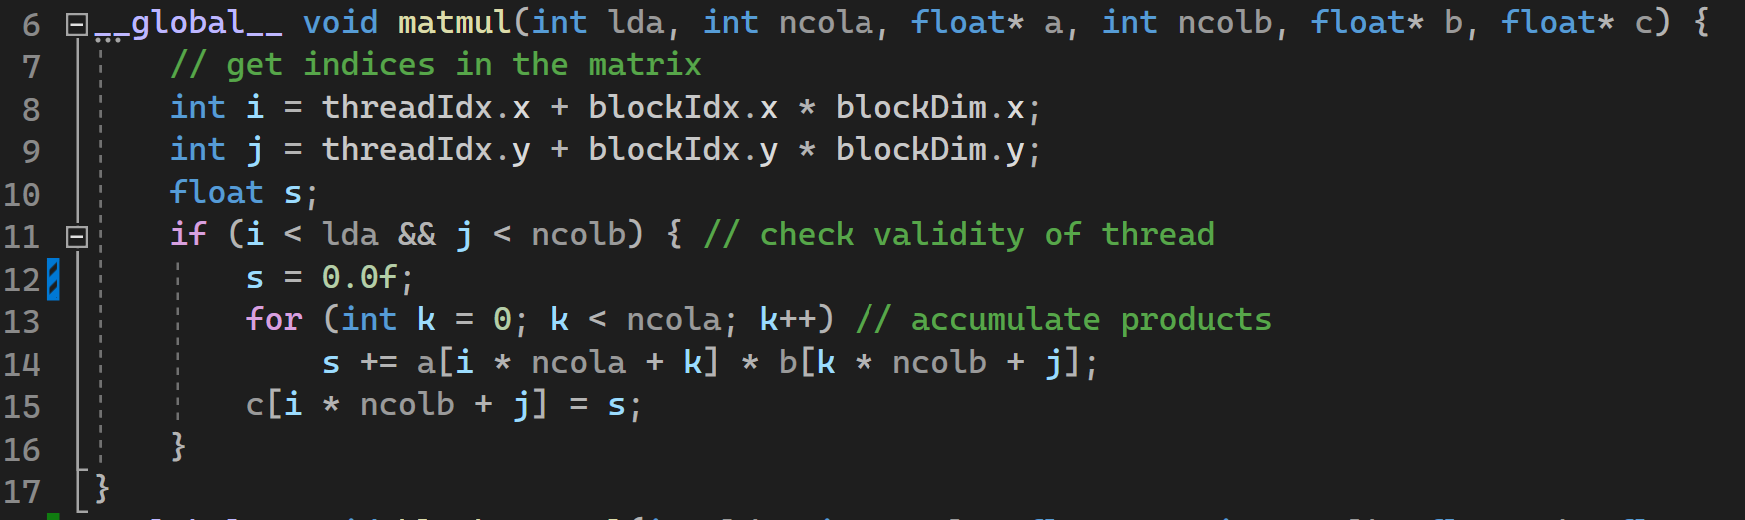
\includegraphics[scale=0.5]{matmul.png}
   \end{figure}
   \begin{itemize}
    \item<+-> L'élément à calculer est obtenu à partir des coordonnées de bloc (\texttt{blockIdx}), puis de processus
    (\texttt{threadIdx}).
    \item<+-> Seule la boucle interne est conservée.
    \item<+-> Chaque processus opère sur une ligne et une colonne de la matrice
   \end{itemize}
\end{block}
\end{frame}

\begin{frame}
    \frametitle{Exemple de programme}
\begin{block}{Exécution}
   \begin{figure}
    \centering
   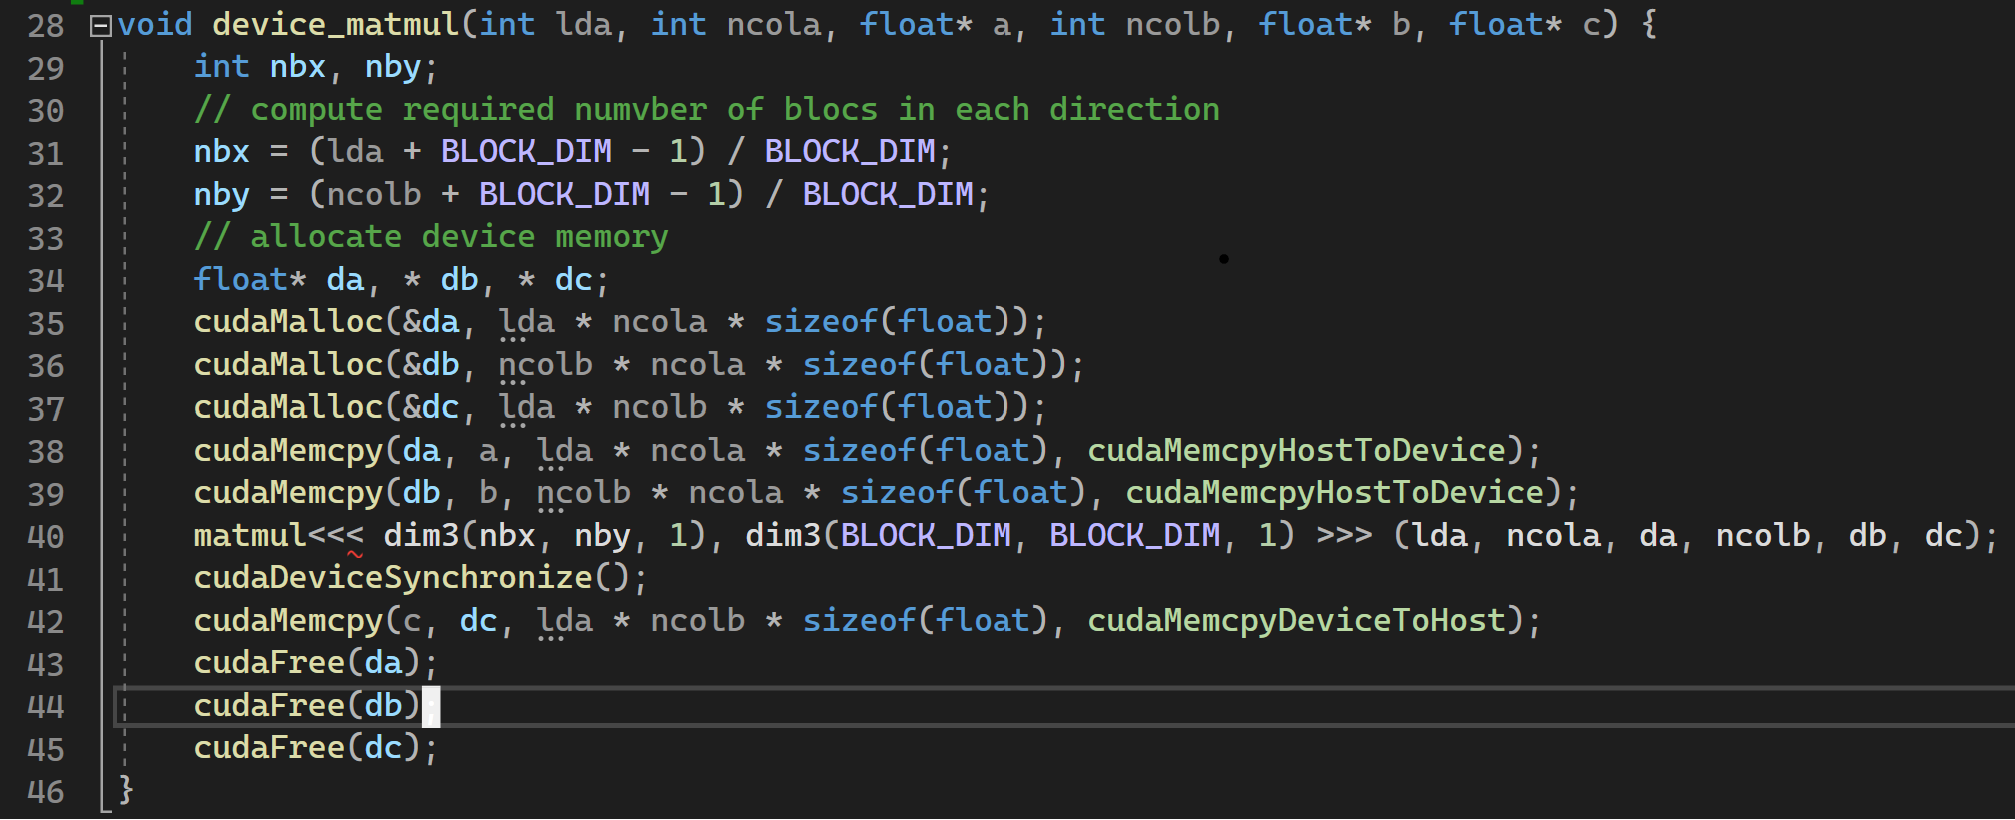
\includegraphics[scale=0.45]{device_matmul.png}
   \end{figure}
   \footnotesize
   \begin{itemize}
    \item<+-> La fonction \texttt{cudaMalloc} permet d'allouer de la mémoire sur le GPU.
    \item<+-> Elle est libérée par \texttt{cudaFree}.
    \item<+-> Les données sont transférées par \texttt{cudaMemcpy}.
   \end{itemize}
\end{block}
\end{frame}

\begin{frame}
    \frametitle{Exemple de programme}
\begin{block}{Vitesse d'exécution}
   \begin{itemize}
    \item<+-> Deux matrices 1000x1000 sont multipliées.
    \item<+-> Sur la configuration de référence, on relève, pour le GPU, une performance de 157 GFlops.
    \item<+-> Pour le CPU, elle est de 2 Gflops.
    \item<+-> Peut-on améliorer la vitesse de calcul ?
   \end{itemize}
\end{block}
\end{frame}

\begin{frame}
    \frametitle{Produit matriciel simple}
\begin{block}{Accès mémoire}
    \begin{tabular}{cc}
        \begin{minipage}{0.45\textwidth}
 \begin{figure}[htbp]
    \centering
   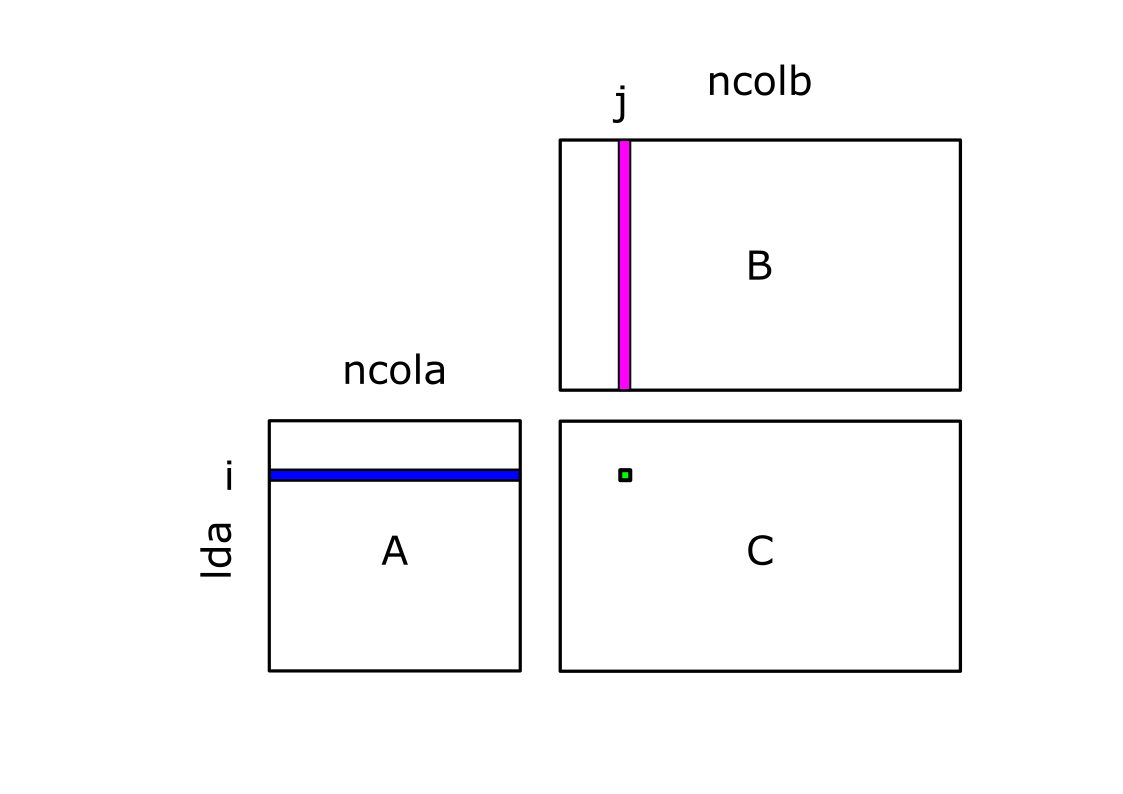
\includegraphics[width=\textwidth]{matmul_simple.png}
    \caption{Accès linéaire.}
    \label{fig:acces_matmul_simple}
\end{figure}
        \end{minipage} & 
        \begin{minipage}{0.45\textwidth}
            \begin{itemize}
                \item<+-> Seule la mémoire globale est utilisée.
                \item<+-> Tous les processus de même numéro de ligne (resp. colonne) accèdent aux mêmes données dans 
                $A$ (resp. $B$).
            \end{itemize}
        \end{minipage}
\end{tabular}
\end{block}
\end{frame}

\begin{frame}
    \frametitle{Produit matriciel par blocs}
\begin{block}{améliorer l'utilisation des données}
    \footnotesize
   \begin{itemize}
    \item<+-> Le produit de deux matrices peut s'effectuer par blocs:
    \begin{equation}
        \label{eq:produit_bloc}
        \begin{split}
         & \begin{pmatrix}
            A_{1,1} & A_{1,2} & \ldots & A_{1,n} \\
            \vdots & \vdots & \vdots & \vdots \\
            A_{i,1} & A_{i,2} & \ldots & A_{i,n} \\
            \vdots & \vdots & \vdots & \vdots \\
            A_{m,1} & A_{m,2} & \ldots & A_{m,n} \\
        \end{pmatrix}
        \begin{pmatrix}
            B_{1,1}  & \ldots & B_{1,j} & \ldots & B_{1,p} \\
            \vdots & \vdots & \vdots & \vdots \\
            \vdots & \vdots & \vdots & \vdots \\
            B_{n,1} & B_{n,2} & B_{n,j} & \ldots & B_{n,p} \\
        \end{pmatrix} \\
        & = \begin{pmatrix}
            C_{1,1} & \ldots & C_{1,p} \\
            \vdots & \vdots & \vdots \\
            \vdots & \vdots & \vdots \\
            C_{m,1} & \ldots & C_{m,p}
        \end{pmatrix}, \quad C_{i,j} = \sum_{k=1} A_{i,k} B_{k,j}
        \end{split}
    \end{equation}
   \end{itemize}
\end{block}
\end{frame}

\begin{frame}
    \frametitle{Produit matriciel par blocs}
\begin{block}{Accès mémoire}
   \begin{tabular}{cc}
        \begin{minipage}{0.45\textwidth}
 \begin{figure}[htbp]
    \centering
   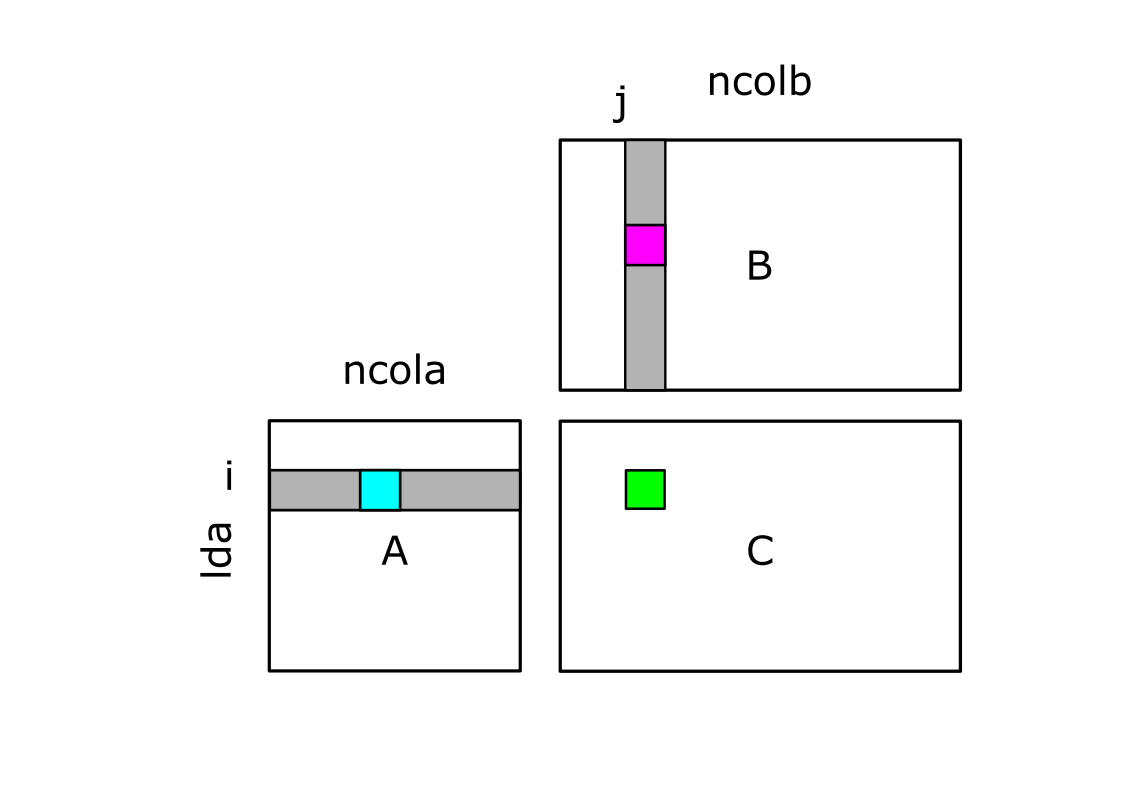
\includegraphics[width=\textwidth]{matmul_bloc.png}
    \caption{Accès par blocs.}
    \label{fig:acces_matmul_bloc}
\end{figure}
        \end{minipage} & 
        \begin{minipage}{0.45\textwidth}
            \begin{itemize}
                \item<+-> Les données d'un même bloc peuvent résider en mémoire partagée.
                \item<+-> Tous les processus d'une même chaîne peuvent effectuer un chargement simultané.
           \end{itemize}
        \end{minipage}
\end{tabular}
\end{block}
\end{frame}
\begin{frame}
    \frametitle{Produit matriciel par blocs}
\begin{block}{Codage}
   \begin{tabular}{cc}
        \begin{minipage}{0.45\textwidth}
 \begin{figure}[htbp]
    \centering
   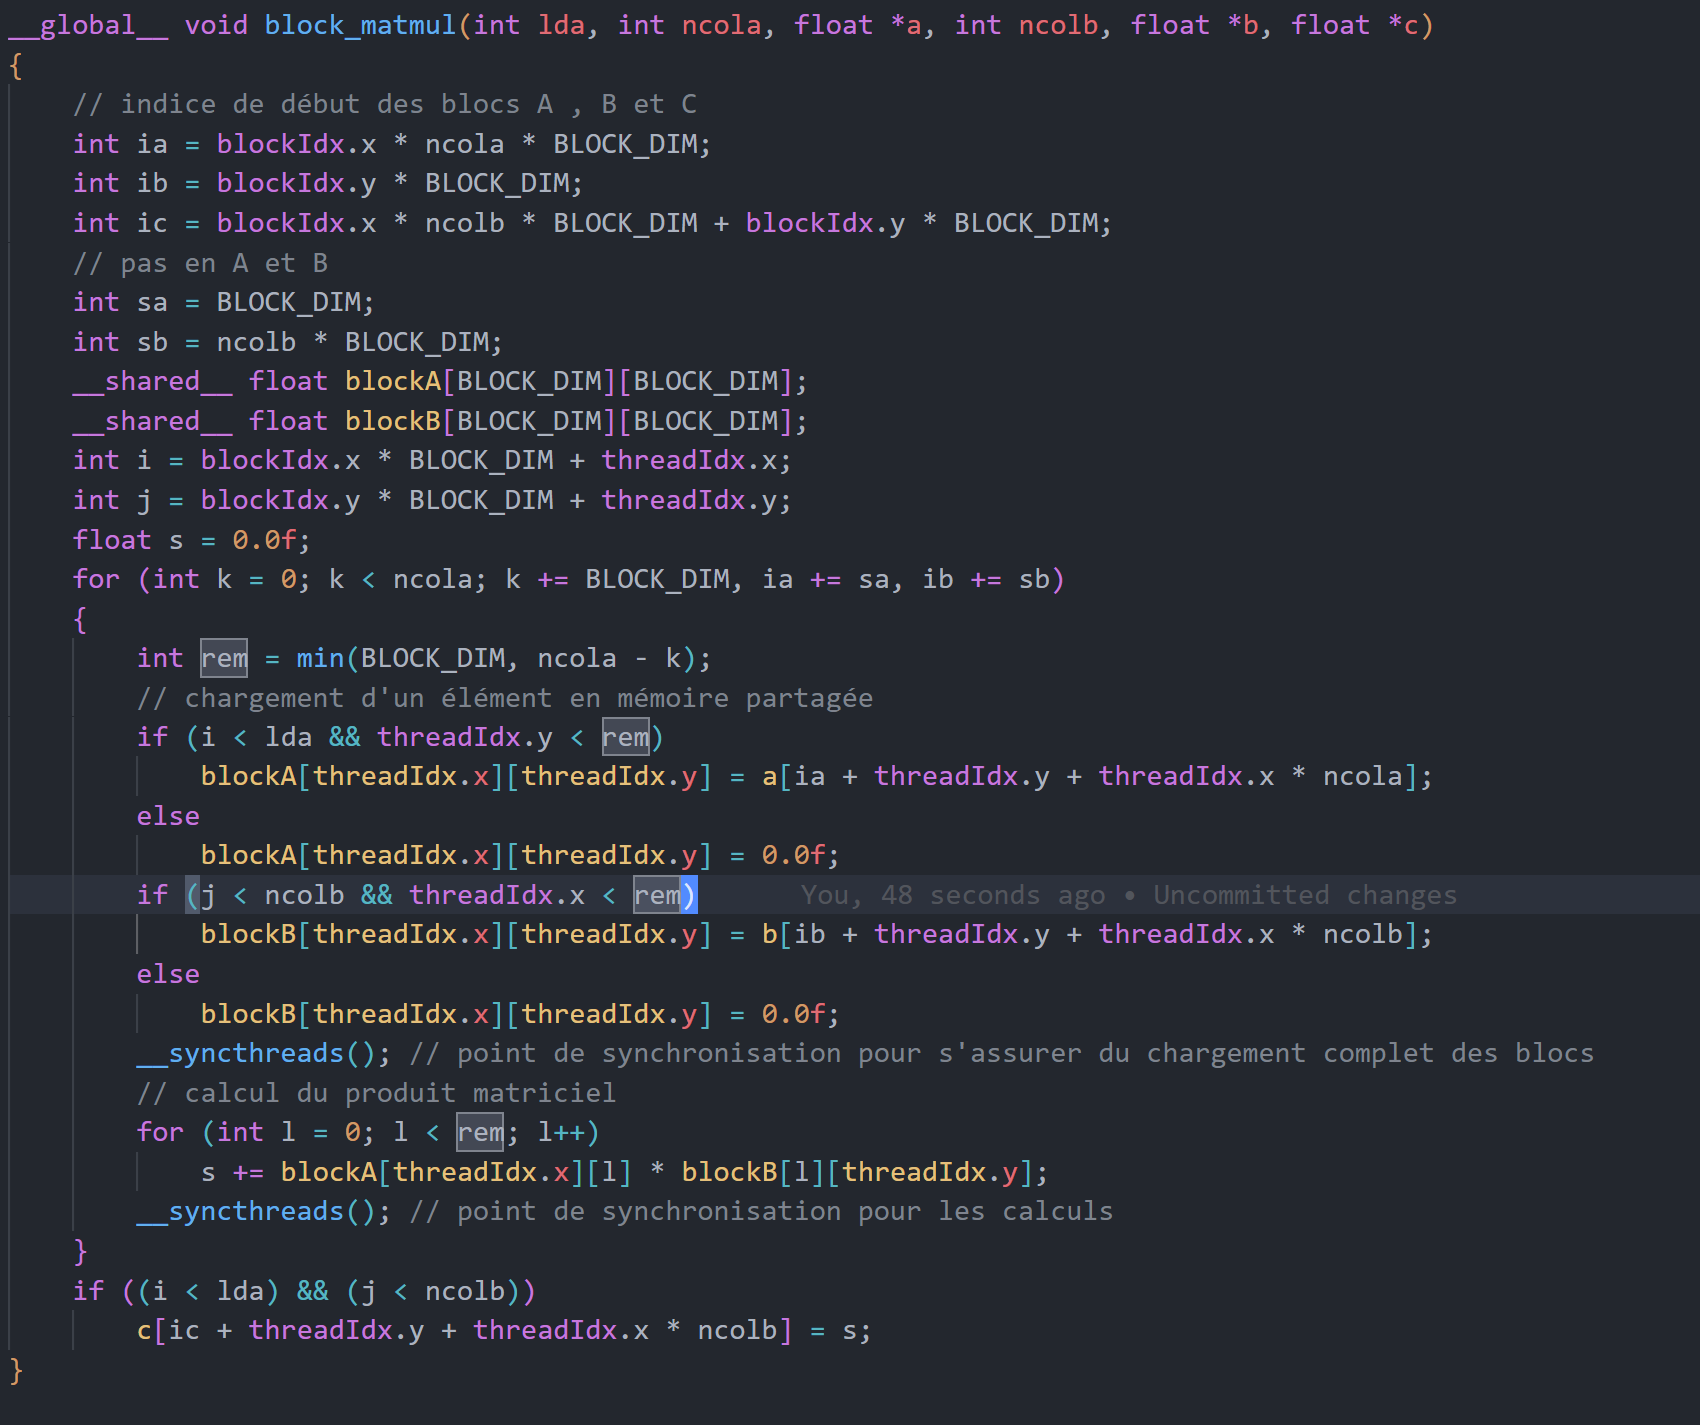
\includegraphics[width=\textwidth]{produit_bloc.png}
    \caption{Accès par blocs.}
    \label{fig:codage_produit_bloc}
\end{figure}
        \end{minipage} & 
        \begin{minipage}{0.45\textwidth}
            \begin{itemize}
                \item<+-> Chaque processus charge un élément en mémoire partagée.
                \item<+-> Les éléments invalides sont mis à 0.
                \item<+-> Les blocs externes sont traités spécialement.
           \end{itemize}
        \end{minipage}
\end{tabular}
\end{block}
\end{frame}
\begin{frame}
    \frametitle{Produit matriciel par blocs}
\begin{block}{Performances}
 \begin{itemize}
    \item<+-> Avec une dimension de bloc de 8 (soit 64 processus), on atteint 350 Gflops sur des
    matrices de taille 10000.
    \item<+-> En comparaison, le CPU ne dépasse pas 2 GFlops, valeur à relativiser, car aucune optimisation n'a
    été appliquée.
    \item<+-> Il est possible d'accélérer encore le code, en particulier en améliorant la gestion des blocs
    situés en périphérie de la grille.
    \item<+-> Le produit matriciel est toutefois un exemple simple, le code GPU étant assez similaire à son 
    homologue CPU.
 \end{itemize} 
\end{block}
\end{frame}
